\documentclass{IEEEtran}
\IEEEoverridecommandlockouts
%% The preceding line is only needed to identify funding in the first footnote. If that is unneeded, please comment it out.
\usepackage{amsmath,amssymb,amsfonts}
\usepackage{algorithmic}
\usepackage{graphicx}
\usepackage{textcomp}
\usepackage{xcolor}

\usepackage{biblatex}
\addbibresource{references.bib}
 


\begin{document}

\title{Co-ordination and co-existence of WiFi at 5GHz}
%----- Note 1: Please check the notes below while you pick a title
% Please find your titles different than the topic names we provided to you
% Functions of a good title:
% it predicts content. 
% it catches the reader's attention. 
% it reflects the tone or slant of the piece of writing.
% it contains keywords that will make it easy to access by a computer search. 
% Avoid too long, too short titles
% too long: unnecessary words
% too short: very broad, does not tell the reader what really is in the paper
% Brainstorm before you write


\author{
\IEEEauthorblockN{Abdullah Abdul Malik}
\IEEEauthorblockA{\textit{389800}, abdullah.amalik07@gmail.com} \\
\and
\IEEEauthorblockN{Binda Liu}
\IEEEauthorblockA{\textit{399167}, liubinda@live.com} \\
\and
\IEEEauthorblockN{Mohammed Mesto}
\IEEEauthorblockA{\textit{390017}, Mohamedmesto111@gmail.com} \\
\and
\IEEEauthorblockN{Yuzhen Li}
\IEEEauthorblockA{\textit{405843}, lyz200495@gmail.com} \\
}


\markboth{TKN WS18/19 SE Network Technologies (L999), Summer 2019}{your name} %!PN


\maketitle

\begin{abstract}
Increased number of  technologies which use the same unlicensed frequency spectrum often cause severe degradation in the performance of these technologies. In this paper we will discuss the technologies that use the 5GHz frequency band. More and more participating technologies in the 5GHz band cause interference with each other which causes the corresponding technologies to face lower performance in their normal operation. We will discuss the possible challenges we face and their solutions in the coordination of WiFi operating at different frequencies e.g WiFi at 2.4GHz and WiFi at 5GHz. We further discuss the challenges and their solutions in the coexistence of WiFi at 5GHz with LTE-U and LAA. Wherein we will discuss also the deployment of LTE technologies coexisting with WiFi technologies in the unlicensed spectrum 5 GHz. Listen before talk (LBT) functionality is required in unlicensed band in order to ensure the fair coexistence among different operators. We propose a LBT enhancement algorithm with contention window size adaptation for LTE with Licensed-Assisted Access (LTE-LAA) in order to achieve not only channel access fairness but also the QoS fairness. In the last part of the paper we explore further to discuss the cross technology communication which enables distinct participating technologies to effectively communicate with each other to optimize the performance.
\end{abstract}

\begin{IEEEkeywords}
WiFi, Virtualization capable WiFi, NFV, LAA, LTE-U, CTC, LtFi
\end{IEEEkeywords}

\section{Introduction}


Wireless local area network is used by devices to access internet and communicate with each other in small areas. Devices connect to a router or access point(AP) through IEEE 802.11 protocol without the help of wired medium. 

Technologies like cellular networks, Internet of Things(IoT) and machine to machine communication (M2M) are causing an increase in the Wireless traffic, because more and more devices are being connected using the above mentioned technologies. In the last decade there is  more internet traffic, which has been transported by WiFi networks than their wired counterparts. It is expected that the WiFi devices will take over 56.8 percentage of internet traffic by 2022 \cite{cisco2018cisco}. With an ever increasing number of WiFi end-users, it is needed that the existing WiFi technologies should be optimized. On the other hand, the WiFi technology itself has also evolved over the years. According to Cisco's white paper, the average WiFi network connection speed was 24.4 Mbps in 2017, and it will exceed 54.2 Mbps by 2022 \cite{cisco2018cisco}. Besides IEEE 802.11 standard protocol, new version of WiFi standard is also introduced, 802.11ax, which is designed to operate in all band spectrum between 1 to 7GHz which also includes the existing 2.4GHz and 5GHz. In order to avoid the interference among the neighboring devices and to improve the efficient utilization of the spectrum, the operation band spectrum certainly will move from 2.4GHz to 5GHz or even higher band.

At the moment these technologies in general and WiFi in particular are not able to effectively use these spectrum resources. For example in case of residential WiFi, all WiFi channels are not used. Or in a high density environment, there are large number of access points(APs). This causes an under-utilization of these precious spectrum resources.

Furthermore according to requirement of Harmonized European Standard in ETSI EN 301 893 Vl.7.1 (2012–06) , LBT grants performing a clear channel assessment (CCA) prior to a new transmission and occupying the channel with limited duration after successful access in the load based equipment (LBE).

These need to devise a plan and come up with the ideas that enable the effective utilization of these scare resources. We are going to discuss a variety of strategies that will enable co-operation of WiFi at 2.4GHz with WiFi at 5GHz and also co-existence of WiFi at 5GHz with other wireless technologies like LTE-U and LAA. Therefore, a critical element of the design for LTE in unlicensed band is to ensure LTE-LAA co-exists with current access technologies such as WiFi on fair and friendly bases.


All of that can enhance the utilization of these spectrum resources and optimize the system performance.

The rest of the paper is organized as follows. Section II gives some basic background of the relative technologies. Section III discusses the internal coordination of WiFi system. Section IV will cover the WiFi network coexists of LET-U ,while Section V presents the coexistence with LAA and some enhanced algorithm.Follows by some ideas of cross communication technology in Section VI.

\section{Background}
In this section we will talk about the background of all the major technologies involved. First we will talk about the WiFi technology and their different standards which are in use right now. Secondly we will talk about the LTE technology and its variant which operates in the unlicensed frequency band i.e LTE-U. We will also go through the different access mechanisms that these technologies use and the their comparisons with each other.

\subsubsection{WiFi networks}

\graphicspath{{Images/}}
\maketitle
\begin{figure}[htp]
\centering
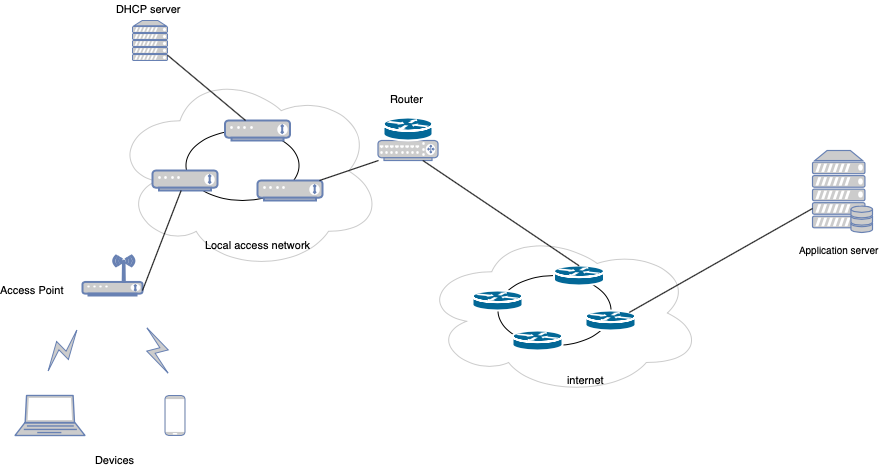
\includegraphics[width=8cm]{tkn-report/Images/wifi.png}
\caption{Basic architecture of WiFi network}
\label{wifi-architecture}
\end{figure}

WiFi is one of the radio technologies which is based on the IEEE 802.11 standards. It is used for the wireless local area networking. The WiFi networks can be an infrastructure network, which has a fixed central element (base station, access point). This kind of network’s structure has a common backbone. Meanwhile it can also construct an independent network with which the elements in the network can directly connect to each other (Ad-hoc network). Basically the WiFi system is a distributed network, the classic architecture is shown in the figure \ref{wifi-architecture}.

In Medium Access Control (MAC) of WiFi network, WiFi stations(STA) cannot detect collisions, when collision happens, it will waste the whole frame. To avoid collisions, we need to use some back-off procedures where a channel is reserved. We can have this capability by using a method called Carrier Sense Multiple Access with Collision Avoidance (CSMA/CA). In CSMA/CA, the WiFi STAs will sense the channel before transmission, waiting for free medium and then transmitting the frame. It will send a short packet for channel reservation, which are called Request to send (RTS) and Clear to send (CTS). RTS is used by the sender to check the availability of the receiver. Once RTS is reached at the receiver side. If the receiver is idle at that time it will reply with a CTS packet. Once the CTS packet is reached at the sender, the channel is reserved, and data can be transmitted reliably. If there is any collision, it will stop transmission immediately. After waiting for a random back-off time, it will re-transmit. The key rule of the CSMA/CA is back-off before collision. The operation of the CSMA/CA is shown in the figure \ref{csma-operation}. In the problem of WiFi network resource sharing, we normally use Distributed Coordination Function (DCF). When a station wants to transmit, DCF will require it knows the channel status for a DIFS interval. The CSMA/CA random back-off time is preventing the collision among the waiting time, it can be called contention window. DCF protocol is in principle fair, and it assume that the contention window is set a minimum value in first transmission and double up to a maximum value after each transmission failure\cite{Tinnirello2011}.

\graphicspath{{Images/}}
\maketitle
\begin{figure}[htp]
\centering
\includegraphics[width=8cm]{tkn-report/Images/csam:ca.png}
\caption{Basic CSMA/CA operation}
\label{csma-operation}
\end{figure}


When the STA needs to connect to a WiFi network, it could search a suitable channel by using different way, passive or active scanning. After finding the network, STA should use a shared key (WEP) to authenticate, and then associate with an access point. The AP gives the STA an IP address by DHCP server.

\subsubsection{Coexistence LTE-U and 5GHz WiFi }

Nowadays with exponentially increasing requirements of data, the frequency band of LTE has been extended from the licensed spectrum into an unlicensed spectrum. Meanwhile, this 5GHz available unlicensed radio band is initially used by WiFi 5GHz devices. It is well known that LTE is a communication standard that has been developed by 3GPP \cite{BenHafaiedh2018a} and it uses a centrally scheduled mechanism to ensure the performance in a licensed spectrum. By contrast, WiFi is built on distributed carrier sensing multiple access with collision avoidance (CSMA/CA), where the carrier sensing mechanism allows transmissions only when the channel is sensed as idle. Hence, due to the difference about the access mechanism between the LTE-U (centralized) and WiFi (decentralized), when both users of LTE-U and WiFi compete in the same unlicensed frequency band, the LTE-U users may occupy too many resources in the spectrum and it may also cause the WiFi 5GHz users to be unable to access the channel. Therefore, it is necessary to study the coexistence of LTE-U and 5GHz WiFi. In other words, a novel mechanism for this kind of coexistence, which is not harmful to the existing protocols, is needed.

To solve these problems some approaches have been previously existing and they can be taken into two main categories:
\begin{itemize}
    \item LBT-based solutions
    \item Carrier Sensing Adaptive Transmission (CSAT) based solutions
\end{itemize}
 With the LBT mechanism, when LTE-U users want to transmit, they must at first detect whether the channel idle or not. If the unlicensed spectrum is busy, SBS will go back a period time. But LBT scheme has several flaws. For instance, if there are multiple WiFi users in a dense environment, the LTE-U users will have rare opportunities to access the channel. Thus, the performance of coexistence will highly decrease. There are also limitations for different markets such as China and India are in non-LBT market. Compared to LBT, CSAT-based schemes have gained popularity because they do not require any changes to existing LTE protocols. For the CSAT mechanism, it defines a transmission cycle in which LTE-U only uses a part of the time interval for data transmission, where in the duty cycle of transmission execution and transmission stop is the activity of other transmission systems in the cell. The degree is determined so that the sharing of channels and the quality of services can be ensured. They adjust the values to adapt and select the duty cycle. In this case, the performance can be optimized meanwhile the fairness of coexistence of LTE-U and WiFi 5GHz may be also realized. Besides, 3GPP has not yet standardized LBT for LTE-U. In section 4 we discuss the non-LBT solutions in detail.


\section{WiFi network Coordination}
The IEEE 802.11 WiFi system operates on the unlicensed spectrum (ISM), and now mainly on the 2.4GHz and 5GHz frequency band. With the increasing WiFi devices and end-users, 2.4GHz ISM band is already crowded, So 5GHz band offers the opportunity in this scenario. In this section, we will focus on several scenarios of internal coordination of WiFi network, where WiFi devices operating at different frequency bands can co-ordinate with each other, which can improve its system performance and the efficiency of the spectrum utilization.

\subsection{Challenges}

The WiFi network is becoming crowded, in the real WiFi systems, massive end-user devices and access points(APs) connect into the WiFi system(figure \ref{massive}), which we call density WiFi environment, it can cause the decreasing of the system performance\cite{Bhalla2016}. Furthermore, the WiFi system itself also has some problems which can degrade the system efficiency. We will discuss them below.

\graphicspath{{Images/}}
\maketitle
\begin{figure}[htp]
\centering
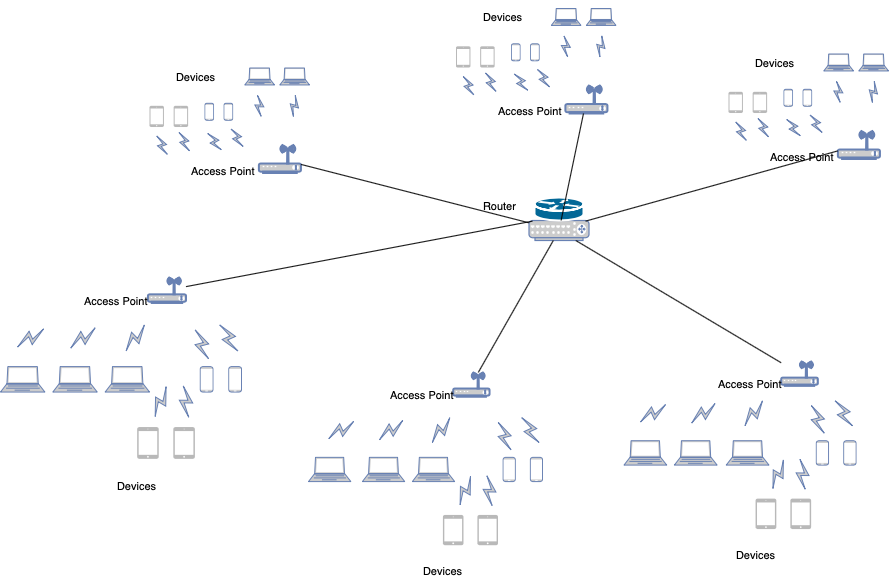
\includegraphics[width=9cm]{tkn-report/Images/meshaps.png}
\caption{Massive connection of WiFi system}
\label{massive}
\end{figure}

\subsubsection{Hidden terminal problem}
The hidden terminal problem is a much more difficult problem caused by WiFi devices than the direct channel competition\cite {Park2014}. When two nodes or stations will communicate with a wireless access point (AP), they can directly sense the AP, but cannot notice each other, this leads to difficulties in medium access control sub-layer. As shown on the figure \ref{hidden}, when two stations(STAs) want to send a packet to the access point, STA1 sends a packet to the AP directly, meanwhile STA2 wants to also send a packet to the AP, however it doesn't know the STA1 is sending the packet at the same time. This causes collision.

\graphicspath{{Images/}}
\maketitle
\begin{figure}[htp]
\centering
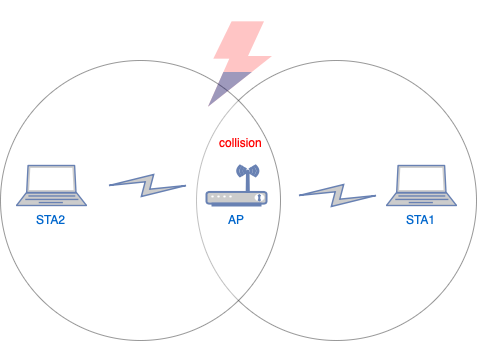
\includegraphics[width=8cm]{tkn-report/Images/hidden.png}
\caption{Hidden terminal problem}
\label{hidden}
\end{figure}

\subsubsection{Adjacent channel interference}
With more and more end-users in WiFi networks, they will occupy different channels. When there are too many APs arranged too closely, that means more than one adjacent channels are being used at the same time. For example 4 channels can be used at the same time in same area of the frequency, and several of them would be overlapping. In order to transmit more efficiently, it is better to let the APs communicate on non-overlapping channels.


\graphicspath{{Images/}}
\maketitle
\begin{figure}[htp]
\centering
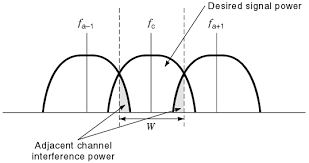
\includegraphics[width=8cm]{tkn-report/Images/overlapping.jpg}
\caption{Adjacent channel interference}
\label{ACI}
\end{figure}

Here we have 3 closely arranged devices use the Channel 1,2 and 3 (figure \ref{uplink}).Even if the transmission spectrum is perfectly shaped from the viewpoints of the standard or radio regulation, the received up-link packets at an AP from a STA can be interfered with the adjacent channel interference (ACI) power from the closely arranged AP directly.\cite{Shoji2014}

\graphicspath{{Images/}}
\maketitle
\begin{figure}[htp]
\centering
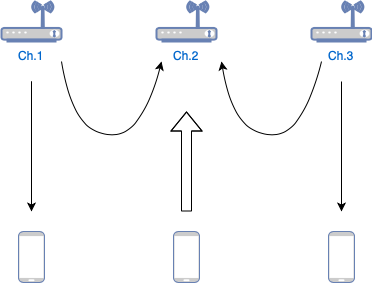
\includegraphics[width=8cm]{tkn-report/Images/uplink.png}
\caption{Up-link packets interfered by the ACI from the closely arranged APs
}
\label{uplink}
\end{figure}
 
 On the other side, for the down-link procedure. Each AP will conduct the carrier sense before transmitting its down-link packets and determine if the channel is busy or idle. When the APs are closely arranged, the ACI power received at APs could reach the threshold level(figure \ref{downlink}). That could cause the malfunction of the carrier sensing procedure, even if the channel is actually idle. Thus the AP needs to wait a random time to avoid "collision". 

\graphicspath{{Images/}}
\maketitle
\begin{figure}[htp]
\centering
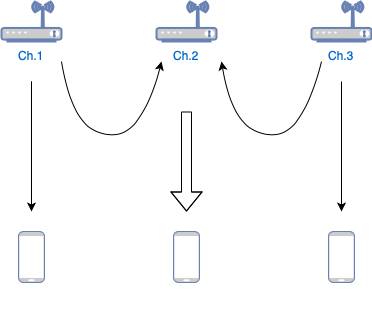
\includegraphics[width=8cm]{tkn-report/Images/downlink.png}
\caption{Down-link packets disturbed by miss-decision of carrier sense due to the ACI from the closely arranged APs
}
\label{downlink}
\end{figure}


\subsection{Solutions}
WiFi system could be optimized by the system internal coordination. To provide interference free environment and at the same time, to get higher system performance, some suitable coordination strategies can be implemented. In this paper we will discuss about following strategies:


\subsubsection{Virtualization capable WiFi}
Virtualization is a very important concept of network design in 5G network, we could also consider implementing it in WiFi system. There are two main methods in this scenario, Network Function Virtualization (NFV) and Software Defined Networking (SDN). NFV enables network functions that were traditionally tied to hardware appliances to run on cloud computing infrastructure in a data center. SDN is an architecture where the control and data planes are decoupled, network intelligence and state are logically centralized, and the underlying network infrastructure is abstracted from the application.Virtualization capable WiFi is a centralized solution to optimize the WiFi network by the internal coordination (figure \ref{VNF}).

\graphicspath{{Images/}}
\maketitle
\begin{figure}[htp]
\centering
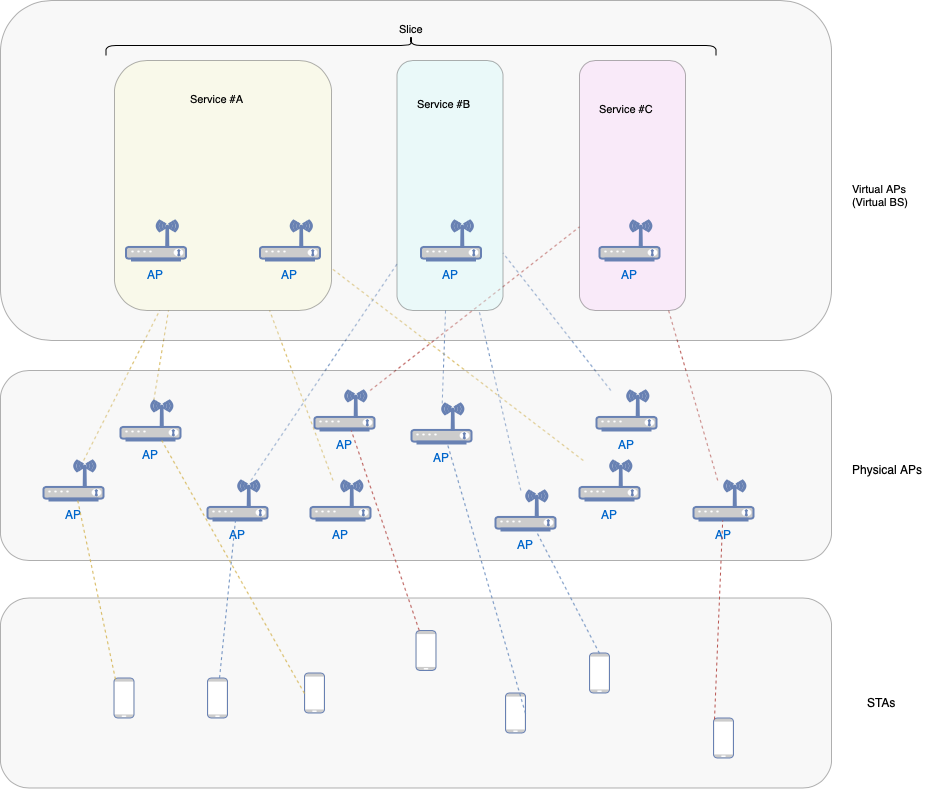
\includegraphics[width=9cm]{tkn-report/Images/VNF.png}
\caption{the virtualization of WiFi network}
\label{VNF}
\end{figure}

\paragraph{Network Model}
Very similar to 5G network, the virtualization of WiFi network is achieved by abstracting some parts of physically available WiFi network resources. That means to build a virtual network on top of the physical WiFi networks regardless of their physical structure. Allocating the independent parts called slices of resources only for a specific service or application. And the management of severs or applications are fully programmable. Such as making the configurations, the settings, and the algorithm to operate the abstracted resources.

\paragraph{Logical Model}
In general, a logical integration approach could be used. That means there are multiple physical APs which are logically integrated into a single virtual AP. They could act in co-ordination as one single AP. Virtual AP could be configured independent of physical structure of WiFi network. So when a STA connect to a physical AP, that means it associates with the virtual AP which consists of multiple physical APs.

\paragraph{Dynamic Configuration}
In a virtual WiFi system, we could use dynamic configuration to select channel and against probe request frames \cite{Nakauchi2014}. One example is shown in the figure \ref{configuration}. Each virtual BS works on only one single interface, regardless of how many physical APs it actually has. That could make the virtual BS configurable with the same MAC address, BSSID, ESSID. All the beacon frames can be transmitted with the same beacon frame data. By controlling the virtual BS with the specific algorithm, the transmission channel within the virtual BS could be dynamically selected.

Probe request and probe response is a basic function in IEEE 802.11. To establish the connection, STA will transmit probe request for target ESSID using different channels one by one. As shown in the figure\ref{configuration}, STA belongs to slice 2, in this procedure, vBS 2 responds to the probe request. Virtual BS 2 has two APs which operate on Channel 11 and Channel 7. The manager of the vBS 2 knows which AP is occupied by less STAs, which channel is better performance, then the AP 3 is chosen for the  probe response.

In this way, closely arranged APs could have more chance to use a better channel without the ACI.


\graphicspath{{Images/}}
\maketitle
\begin{figure}[htp]
\centering
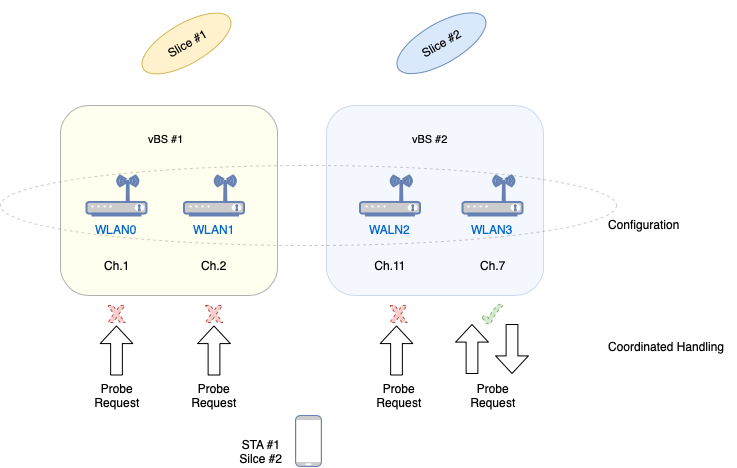
\includegraphics[width=9cm]{tkn-report/Images/configuration.png}
\caption{Dynamical configuration}
\label{configuration}
\end{figure}


\subsubsection{Radio Resource Management Based on Radio Environmental Maps}
The Radio Resource Management (RRM) is a data-set of spectrum occupancy and interference levels computed based on raw spectrum measurements, propagation modeling and spatial interpolation algorithms \cite{Rakovic2016}. Radio Resource Management (RRM) algorithms can use Radio Environmental Maps (REMs) to optimize the overall network performance. REM is an essential technology to optimize the usage of spectrum bands. The radio interference levels, propagation models, transmitter locations, communication parameters and performances of the underlying communication devices, these kinds of distinct data can be processed. Furthermore the REM data could provide insight for the interference management and coordination process for WiFi end devices fostering optimal RRM in ISM band.

In this paper we will not discuss more details about this scenario, there are some experiment in\cite{Dion2017},and some other scenario to optimize WiFi system in \cite{Tinnirello2011},\cite{Molina2017}.


\section{Coexistence of WiFi 5GHz with LTE-U}
In the previous section background, we have briefly introduced the differences between LTE-U and WiFi mechanisms. In this part, we will first focus on the mechanism of LTE-U, and then find three sets of solutions from different perspectives, that is, how to connect LTE-U to the existing WiFi spectrum, and how to make them work together to achieve efficient and fair coexistence at the same time.

LTE now supports a capability called carrier aggregation. It is intended to allow mobile operators to combine the various licensed spectrum bands they own into a single data connection between the user and the network. Licensed spectrum is highly efficient due to its exclusive occupancy of the spectrum, but the amount of available licensed spectrum can be limited and costly. In carrier aggregation technologies the secondary cell, which is associated with LTE-U, has been taken into use. However, we must consider the existing WiFi users in this band. If the interference can be detected in advance, the coexistence will be more efficient. The following figure 10, which is from the paper\cite{Olbrich2017}, describes the scenario where LTE-U and WiFi are co-located. In this case LTE-U users only transmit in the UL and WiFi transmit simultaneously UL and DL in the BSS, thus, interference in the interactive area is generated.

\graphicspath{{Images/}}
\maketitle
\begin{figure}[htp]
\centering
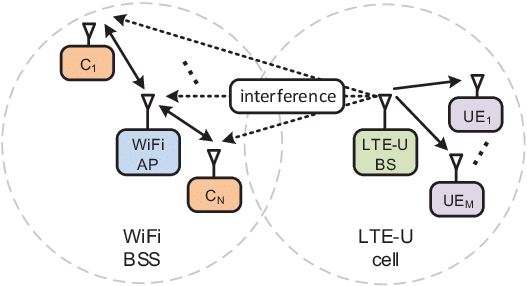
\includegraphics[width=9cm]{interference.png}
\caption{WiFi BSS co-located with LTE-U cell\cite{Olbrich2017}}
\label{interfece}
\end{figure}

Furthermore, we also consider the coexistence from the WiFi perspective. The coexistence of LTE-U and WiFi 5GHz sounds great for mobile network operators, because it has a high potential to increase the capacity of existing LTE networks by utilizing existing infrastructures in the unlicensed band. But WiFi operates 802.11 standards and it is designed to be a cooperative network. It is hard to ensure that, WiFi will not be interrupted by LTE-U when it transmits in a coexistence scenario. In following we give a novel concept called HAP i.e. hyper access point as one kind of solution, which can separately control the performance of WiFi and LTE-U compared with the ordinary WiFi schemes.


\subsection{Challenges}
On a practical and theoretical level, executing the coexistence of  LTE-U and WiFi 5GHz is a very difficult task. First of all, WiFi operates using DCF, which is based on CSMA/CA to sense the channel either it is idle or busy in each time slot. When LTE transmission occurs, it is not able to estimate the transmission of WiFi. Before LAA, LTE-U duty-cycle does not carry out LBT, it can cause poor WiFi throughput performance in some conditions and high interference as well. In this section we will mainly focus on these two challenges as following:

\subsubsection{Fairness for Coexistence}
The first challenge we face is, how to ensure fairness for the coexistence of LTE-U and WiFi 5GHz. When LTE-U and Wi-Fi networks coexist, Wi-Fi faces the situation that the channel cannot be accessed, and the heterogeneous network has no channel to transmit messages. Therefore, how to achieve fair coexistence between LTE-U and Wi-Fi without reducing data throughput efficiency is a key issue that needs to be solved currently. Existing solutions such as CSAT (Carrier Sensing Adaptive Transmission) and ABS (Almost-Blank-Subframes) provide a guarantee of both efficiency and fairness. In the following part, we will also focus on other approaches.

\subsubsection{Higher Efficiency}
The second challenge we should solve is, how to make the coexistence more efficient. To avoid WiFi be interrupted by LTE transmissions we should set up a new coordination structure. The main idea behind this is, that LTE-U and WiFi users work in a dynamic scheduling pattern. In the following solutions, we propose a new concept namely HAP, which allows LTE-U to efficiently access the unlicensed spectrum of WiFi, and can make good use of the cooperative mechanism of WiFi to dynamically allocate resources to different users and coexistence scenarios. Finally, the efficiency of the system will be greatly optimized. We will talk about with more details in the corresponding solutions.

\subsection{Solutions}
In this section, three groups of coexistence design schemes are proposed to solve the coexistence problem between LTE-U and Wi-Fi.

\subsubsection{HAP}
HAP means a novel Hyper Access Point\cite{Chen2016}. Unlike traditional existing LTE-U mechanism, HAP can serve as both LTE-U SBS and WiFi AP as one node and operates as a kind of coordination pattern. It can utilize two standard WiFi MAC protocols, namely PCF (Point Coordination Function) and HCF (Hybrid Coordination Function). In a heterogeneous network, traditional APs and new HAPs operate on the same unlicensed spectrum. We can see this problem i.e. how to allocate resources to different users, as to how to obtain a dynamic optimal allocation of CFP and CP. However, CFP means centralized cooperation, and CP stands for traditional CSMA/CA mechanism. The following figure\ describes this HAP MAC frame. Each work cycle is divided into CFP and CP. In the CFP time slot, the beacon frame is sent first, and then the LTE-U will be transmitted in the form of central control, while other LTE-U users and WiFi users temporarily stop transmitting until the start of the CP time slot, and the WiFi user starts transmitting. .

\graphicspath{{Images/}}
\maketitle
\begin{figure}[htp]
\centering
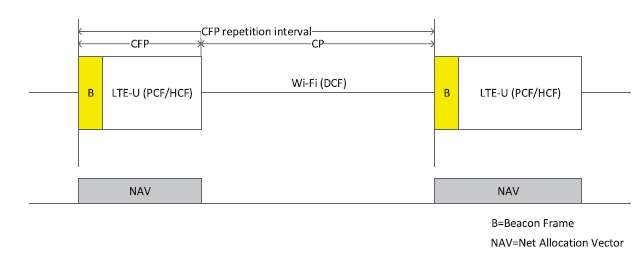
\includegraphics[width=9cm]{tkn-report/Images/HAP.png}
\caption{HAP frame structure\cite{Chen2016}}
\label{interfece}
\end{figure}

HAP has many advantages. For example, it is obvious that after different unlimited resources are allocated to different users, the interference will be greatly reduced because the transmission of LTE-U and WiFi has been completely separated. They exist independently and do not interfere with each other. Therefore, the utilization and management efficiency of unlimited resources have been greatly improved. Besides, the flexible control of the duty-ratio of coexistence.

\subsubsection{Association Fairness}
This scheme is similar to the previous HAP scheme, but more attention is paid to the beacon frame generation mechanism in different situations. Through the paper\cite{Sathya2018}, we know that the maximum duty cycle of LTE-U on idle channels is 95 percentage. When WiFi users want to share the same channel with LTE-U, they must first deliver a beacon frame as described in the previous solution. That's it. But even in a very long duty ratio, the OFF time is very short, so it is difficult to confirm whether the beacon has been successfully sent. In summary, it is necessary to establish correlation fairness, which is about the threshold of the duty ratio, the drop probability of the beacon frame, and so on. Through some mathematical analysis and model simulation, we can compare the throughput of the entire system in different situations.

\subsubsection{Embedding LTE-U within Wi-Fi Bands}
We have already discussed the coexistence mechanism of LTE-U and WiFi. Now we discuss a new approach based on the WiFi perspective, which is to connect LTE-U to the standard WiFi protocol. This approach can greatly improve the fairness and efficiency of coexistence because it does not change the existing WiFi rules. The paper\cite{Chen2017} proposes two different LTE-U access methods, namely UCA TD-LTEmode and standalone LTE-U Operation mode.
In this section, we only discuss UCA TD-LTE, which is the LTE mode of unlicensed carrier aggregation time duplexing. As shown in the following figure, the entire process is divided into an association step and a data transmission step. In the association step, the HAP determines how and when to perform carrier aggregation. The process of carrier aggregation determines the allocation of LTE and LTE-U users. LTE-U users send a beacon frame at the beginning of each cycle, which contains very important information, the length of the CFP. After that, the LTE user will receive the control signal, and the UE can receive the unlimited resource signal.
\graphicspath{{Images/}}
\maketitle
\begin{figure}[htp]
\centering
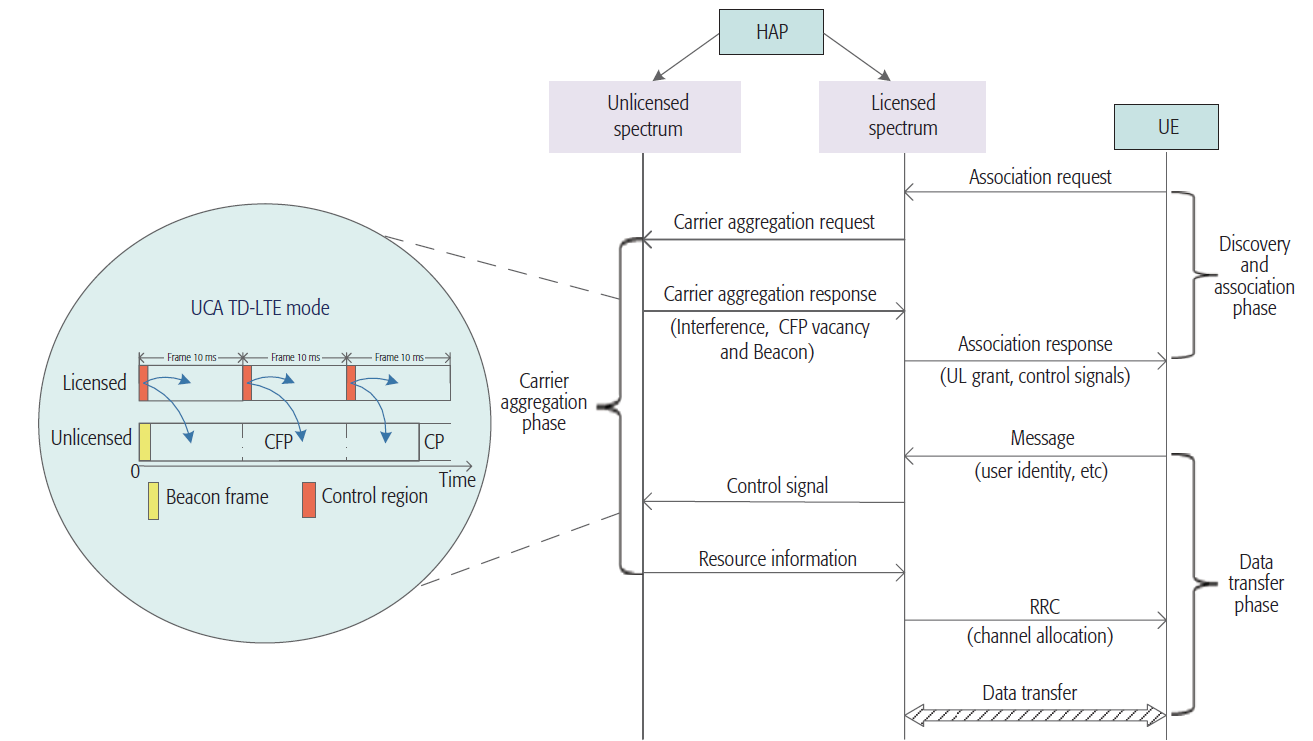
\includegraphics[width=9cm]{tkn-report/Images/UCA.png}
\caption{UCA TD-LTE\cite{Chen2017}}
\label{UCA}
\end{figure}


\section{Coexistence of WiFi with LAA}


\subsection{System Model}

 We will focus here on the coexisting of LTE technologies with Wi-Fi technologies in the unlicensed spectrum 5 GHz. In LTE-LAA, the data service amount expoiting is the most important issue in transmission. The channel availability should be checked before the transmission to guarantees no huge transmission quality impact on other nodes over an unlicensed channel. As specified in [99], the file status in an eNB can be classified into two stages, the buffer state and the backoff state in a LAA system. In this work, we assume a non-saturated condition (the number of arrived files will never exceed the buffer size), which is more general and meaningful. In addition, first come first served (FCFS) algorithm is considered as the stack protocol in this work [1010]. Furthermore, it is assumed that the traffic model for each base station is FTP-3, i.e., the arrival of request files follows an exponential process. Therefore the probability Pk of k-th files entering the buffer can be express as: 
 \begin{equation*}P_{k}=\text{Pr}(X=k)=\lambda\exp^{-\lambda k}, \tag{1}\end{equation*}
  where, λ is the file arrival rate of the eNB.

  \cite{Tao2015}
  
  As we need to model this problem, the file access activities in a LAA eNB are summarized as a Markov chain model in Fig. 13. A file status transits from the buffer state to the backoff state (from T1to bi) when it is scheduled by the eNB. A backoff counter w for the file is firstly generated in the range [0,CW−1] randomly fulfilling the uniform distribution. That means the file has the same probability dropping into the state bi, where i∈[0,CW−1]. In the backoff state, the equipment shall perform a CCA check to observe the channel availability. If the channel is checked as free, the backoff counter can be decreased by 1 (i.e. the file status moves from bi to bi−1). Otherwise, the backoff number maintains the same value since the channel is occupied by other nodes. The transition probability of this process is assumed to be p which is related to the collision rate, is determined by many factors such as the number of competition nodes, the channel condition and the traffic demand of a given node. In this contribution, we assume that backoff transition probability p can be approximated by the channel occupancy rate or sensing results of a given node. For instance, if a historical sensing result of a node is that with 80 percent of the case the channel is sensed as free and with 20 percent of the case the channel is sensed as busy. In this case, p can be approximated to be 4/5. \cite{Tao2015}
  
  
  
  
\graphicspath{{Images/}}
\maketitle
\begin{figure}[htp]
\centering
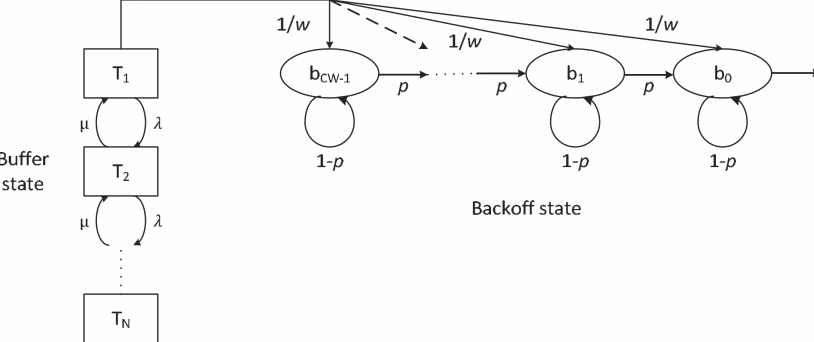
\includegraphics[width=9cm]{tkn-report/Images/Transition_model.png}
\caption{Transition model of file activities in an enb.}
\label{fig:lion}
\end{figure}
  
  
  
  
thus, the summarized of transition probabilities in the whole Markov chain can be: 
  \begin{equation*}\begin{cases}P(\text{b}_{i}\vert \text{T}_{1})=1/w\\ P(\text{b}_{i-1}\vert \text{b}_{i})=p.\\ P(\text{b}_{\text{i}}\vert \text{b}_{i})=1-p \end{cases}\tag{2}\end{equation*}
  
  In this condition, P(Y|X) represents the conditional probability of a transition from state X to state Y. The first equation in (2) indicates a file transits from the buffer state to backoff state, and T1 indicates the latest state when file is ready to be transmitted, w is the backoff counter. The second and the third equations in (2) indicate the transition probability of backoff counter decreased by 1 or not, respectively.
  
  

\subsection{Proposed LBT Procedure Enhancement}

In this section, we elaborate our designs of adjusting contention window size for LBT procedure.
\begin{itemize}
    \item  Quality of service Metric Design
    In this part, we will talk about the average transition duration for backoff counter.
    so at beginning: 
    The transmission latency is a very sensitive QoS index, especially when the real-time service is adopted. In the following, the approximated average transmission delay is deduced and considered as an example of the QoS metric. According to (2), the average transition duration for backoff counter decrease by 1 can be calculated as:
    
    \begin{align*}t_{1-\text{backoff}}&=\lim_{n\rightarrow\infty}(p\cdot t_{\text{slot}}+p\cdot(1-p)\cdot 2t_{\text{slot}}+\notag\\ &\quad p\cdot(1-p)^{2}\cdot 3t_{\text{slot}}+\cdots+p\cdot(1-p)^{n-1}\cdot nt_{\text{slot}})\notag\\ &=\frac{t_{\text{slot}}}{p}\tag{3}\end{align*}
    
    where, tslot is the CCA observation time.

Since the backoff countered w is uniformly generated in the range [0,CW−1]. the average time spend on backoff state can be calculated straightforward:
    
    \begin{equation*}t_{\text{All}-\text{backofff}} = (\frac{t_{\text{slot}}}{p}\cdot \frac{\text{CW}}{2}), \tag{4}\end{equation*}
    
    where, CW is the contention window size. It can be concluded that the average time spend in the backoff state is proportion to CW size and inverse proportion to p.

With above assumptions, the file connection activities can be modeled as MIMII queuing system. According to [11], we can conclude that the average time spend in the system is Ws=1μ−λ Here, λ is the file arrival rate and μ is the system service rate. In this assumption, the service rate is related to the backoff delay and the file transmission time and can be calculated as:
   
   
   \begin{equation*}\mu=\frac{1}{t_{\text{transmission}}+t_{\text{All}-\text{backoff}}}. \tag{5}\end{equation*}
   
    Furthermore, the average time spend in the system of a file can be expressed as: 
    
    \begin{equation*}W_{s}=\frac{1}{\mu-\lambda}=\frac{1}{\frac{1}{t_{\text{transmission}}+(\frac{t_{\text{slot}}}{p})\cdot\frac{\text{CW}}{2}}-\lambda}\tag{6}\end{equation*}
    
    
    For the same type of traffic, the average time spend in the system Ws, which is also can be considered as the average transmission delay, should be maintained at the same level in order to achieve the file connection fairness among different nodes. In this work, the average transmission delay related to the contention window size as shown in (6), are considered as the QoS metric.
   \cite{Tao2015}
    \bigskip
    
    \item\textbf{Adaptive Contention Window (CW) Size Adjustment}  
    
        By gathering the Quality of service (QoS) metric information from neighbor nodes via X2 interface, the node is able to adjust its CW size to achieve service fairness. For example, it is assumed that node A and node B shares the same spectrum resource and has the same type of traffic. If node A approximates its average transmission delay to be 50 ms, and node B approximates its average transmission delay to be 600 ms. By exchange these delay information, node A finds that it performs far better than node B. If a desirable QoS is already achieved by node A, node A could enlarge its contention window value to release some resource to node B so as to achieve fairness between these two nodes. At the same time, node B notices that it does not work in a good situation, it decreases the contention window to grab more channel access opportunity. Furthermore, the QoS metric can be classified into multiple levels due to limited number of exchange information. For instance, the transmission delay can be cataloged into 8 levels, i.e., 3 bits feedback information. The Nodes, that content on the same channel, aim to approach the same level of QoS as shown in Fig. 14. 
    
    
  
\graphicspath{{Images/}}
\maketitle
\begin{figure}[htp]
\centering
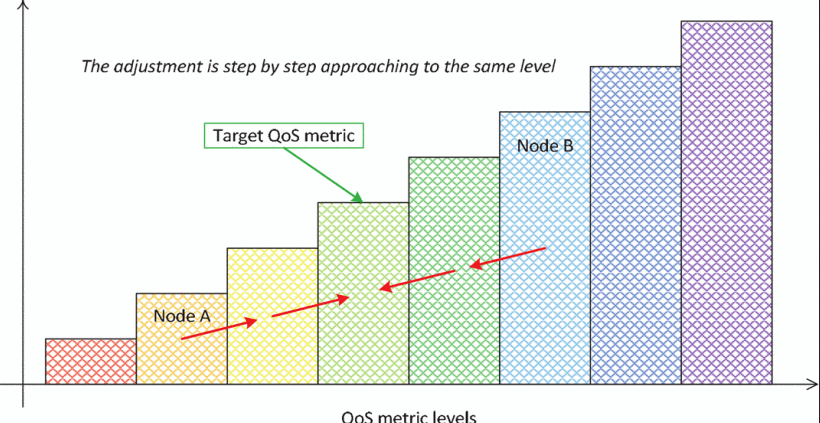
\includegraphics[width=9cm]{tkn-report/Images/Procedure_of_contention.png}
\caption{Procedure of contention window size adjustment.}
\label{fig:lion}
\end{figure}
    
   It has to be mentioned that the CW adjustment should be a semi static and smooth procedure, since slight contention window size adjustment will affect the channel competition result of all contenders and the communication via X2 interface is a relatively slow behavior. For instance, the CW value of each node can be updated every second or tens of seconds, which depends on the speed of information exchange.\cite{Tao2015}

Furthermore, a gradient approaching algorithm is proposed for the CW size adaptive adjustment.

    Firstly, a node collects the QoS metric from nearby nodes to design a target metric. The target QoS metric of a given node can be calculated by averaging all QoS metrics with the same traffic type. Take the average transmission delay as an example:  
    
    \begin{equation*}W_{s}^{avg}=\sum_{i=1}^{N}W_{s}(i)/N, \tag{7}\end{equation*}
    
    where N is the number of neighbor nodes with the same traffic type and Ws(i) is the approximated average transmission delay for node i. In addition, prioritized QoS should be considered in multiservice traffic, e.g., realtime sensitivity service should have better QoS metric than non-realtime service from the fairness point of view.
    
    \begin{enumerate}
    	\item Then, each node compares its own QoS metric with the target metric and selects an appropriate CW value to increase/decrease its own QoS metric approaching to the target one as the following expression:
ifWsi<Wavgs−THCWi=CWi+Step;elseifWsi>Wavgs+THCWi=CWi−Step;elsemaintainCWi;(8)

\begin{align*}&if\,\, W_{s_{i}} < W_{s}^{avg}-\text{TH}\notag\\ &\qquad \text{CW}_{i}=\text{CW}_{i}+\text{Step};\notag\\ &elseif\, W_{s_{i}} > W_{s}^{avg}+\text{TH}\notag\\ &\qquad \text{CW}_{i}=\text{CW}_{i}-\text{Step};\notag\\ &else\notag\\ &\qquad maintain\, \text{CW}_{i};\tag{8}\end{align*}

Here, “TH” is a threshold to trigger the CW size adjustment and “Step” is the adjustment granularity which controls the speed of the adjustment.



        \item By adjusting the contention window size adaptively, the QoS fairness for multiple nodes can be finally achieved.
    \end{enumerate}
  
\end{itemize}



\section{Cross Technology Communication}
In the previous sections we have discussed multiple challenges and their corresponding solutions in order to make both technologies LTE-U and WiFi to coexist in a given scenario. In those solutions we particularly discussed the possible changes in basic working of both these technologies which will ultimately allow them to detect interfering signals and then to efficiently use the spectrum.

Apart from those solutions we are looking towards a scenario where heterogeneous technologies like WiFi and LTE-U can coexist and are able to communicate with each other. We have a possibility of establishing a communication channel between the interfering endpoints operating in different technologies but same frequency bands, and then to communicate with each other so that the interference can be reduced. There are some approaches discussed in the literature about the communication among different technologies, but they generally target the communication between WiFi and other sensor network technologies like ZigBee \cite{Wang2019}, \cite{Yin2017}.But we need a mechanism where we can enable WiFi to communicate with LTE-U. LtFi \cite{Gawowicz2017} provides a solution to make the cross technology communication possible.

LtFi is of low complexity and it is compatible with the WiFi COTS hardware. The only step required is to install a small software on the WiFi AP. LtFi provides the capability to detect the proximity of the nearby WiFi APs. Results from \cite{Gawowicz2017} also show that LtFi is able to perform even at very low signal power level i.e -92dBm. It enables the LtFi to accurately estimate the number of nearby interfering LTE-U BSs.

\subsection{LtFi: Cross Technology Communication system between LTE and WiFi}
LtFi proposes a solution to setup a common channel among co-located WiFi and LTE-U networks. LiFi uses the LTE-U BSs to send the broadcast signals containing the connection and identification data using the air interface. WiFi access points get this data and use it to establish a bi-directional control channel.

\subsection{Challenges}
Currently there is no possibility of discovery component where the co-located WiFi APs and LTE-U BSS can detect the presence of each other. The problem under consideration is to enable the cooperation between co-located LTE-U BSs and WiFi APs operating in the same frequency spectrum 5GHz.

We face two major challenges in order to achieve the desired result. The first is to establish a common management plane between the heterogeneous technologies. The second is cross technology proximity detection i.e to identify the network nodes suffering from performance degradation.

\subsection{Solutions}
The proposed solution in LtFi is to have an architecture where multiple WiFi APs and LTE-U BSs are located in the same area and using the same frequency spectrum. A WiFi AP can be at the intersection of multiple LTE-U rings or it can only be in the vicinity of a single LTE-U BS.

LtFi enables these distinct endpoints to communicate with each other through the protocols which we will discuss in the upcoming sections.

\graphicspath{{Images/}}
\maketitle
\begin{figure}[htp]
\centering
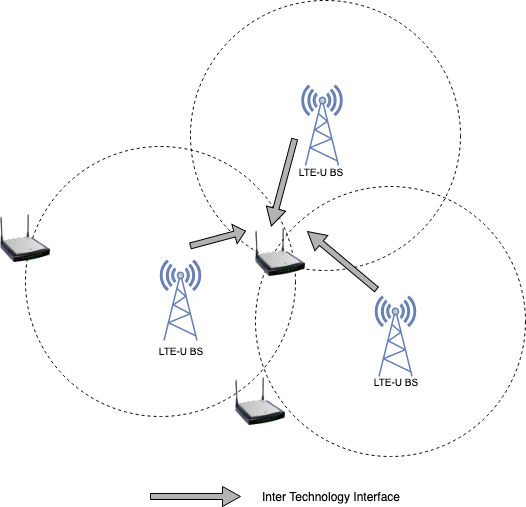
\includegraphics[width=9cm]{tkn-report/Images/LtFiSystemDiagram.png}
\caption{LtFi - System Model}
\label{fig:lion}
\end{figure}

\subsection{System Architecture}
This section explains the architecture of LtFi. LtFi consists of two major components which are as follows,

\begin{itemize}
    \item LtFi - Air Interface
    \item LtFi - X2 Interface
\end{itemize}

\graphicspath{{Images/}}
\maketitle
\begin{figure}[htp]
\centering
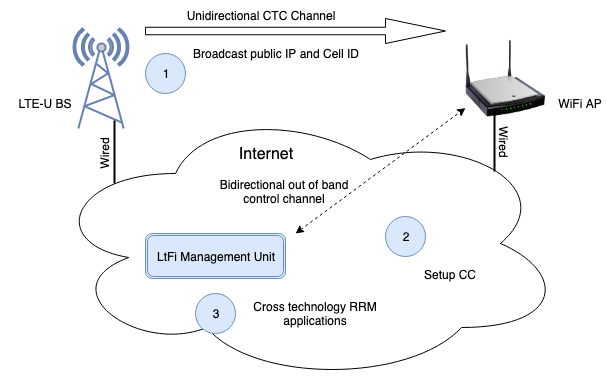
\includegraphics[width=9cm]{tkn-report/Images/LtFiSystemArchitecture.png}
\caption{LtFi - System Architecture Diagram}
\label{architecture-diagram}
\end{figure}

LtFi air interface is used to establish the initial communication channel among LTE-U BS and WiFi AP. As shown in the figure \ref{architecture-diagram} LTE-U station uses the air interface to send the configuration data which is then used by the neighbouring WiFi APs. The configuration data includes the global IP address and the cell id. LtFi makes use of the sub-frame puncturing to insert the data for establishing the cross technology channel. On the WiFi side it monitors the Mac state so that it can differentiate between the WiFi and non-WiFi signals. The same interface is also used for proximity detection.

LtFi- X2 interface is used to establish a two way connection between the corresponding LtFi management unit and WiFi APs over the internet. Once the two way connection is established, the connected endpoints can then share information about the spectrum and interface management.

\subsubsection{Takeaways}
LtFi solves the problem of communication among the heterogeneous technologies but proposing to setup a cross technology channel between participating LTE-U BS and WiFi AP. LtFi is simple to use and works very well with the existing WiFi hardware. The only requirement is to install a small piece of software on the WiFi AP. It requires a simple interface to the LTE-U eNb to send the configuration data to the neighbouring WiFi node, which the WiFi AP later uses to establish over the internet channel with the corresponding LTE-U BS to perform interference and radio resource management. 

\section{Conclusions}
In this paper we discussed the WiFi in general which operates at 5GHz. How we can make the WiFi do some  coordination. We further discussed the LTE unlicensed technology operating on 5GHz and the challenges it puts in coexistence with the WiFi devices working in the same band. By using the Virtualization scenario,the throughput performance of WiFi systems could be improved. This kind of internal coordination of WiFi network could let the system be operated dynamically. The optimized network could adjust different use cases and different network environments. By using the almost-blank sub-frames (ABS) feature to blank a certain fraction of LTE transmissions, WiFi throughput can be effectively increased. In addition to it, a kind of “coordinated structure” should be set up. This is higher-level management of spectrum access between the two systems. We further discussed the cross technology communication between both these technology in order to make the co-existence and co-ordination easy for the participating technologies.

\printbibliography
\end{document}
